\documentclass[a4paper]{article}
\usepackage[14pt]{extsizes} % для того чтобы задать нестандартный 14-ый размер шрифта
\usepackage[utf8]{inputenc}
\usepackage[english, russian]{babel}
\usepackage{setspace,amsmath}
\usepackage{epigraph} % для эпиграфов и продвинутых цитат
\usepackage{csquotes} % ещё одна штука для цитат
\usepackage[unicode, pdftex]{hyperref} % подключаем hyperref (для ссылок внутри  pdf)
\usepackage{amssymb} % в том числе для красивого знака пустого множества
\usepackage{amsthm} % в т.ч. для оформления доказательств
\usepackage[left=20mm, top=15mm, right=15mm, bottom=15mm, footskip=7mm]{geometry} % настройки полей документа 
\usepackage[active]{srcltx}
\usepackage{indentfirst}
\usepackage{listings}
\usepackage{tocloft}
\usepackage{misccorr} 
\usepackage{graphicx}
\usepackage{caption}
\usepackage[style=numeric,sorting=none]{biblatex}
\DeclareCaptionLabelSeparator{defffis}{ --- }
\captionsetup{justification=centering,labelsep=defffis}
\graphicspath{{images/}}
\DeclareGraphicsExtensions{.jpg}
\renewcommand{\cftsecleader}{\cftdotfill{\cftsubsecdotsep}}
\newcommand{\ran}{{\rm ran}\,}
\newcommand{\diag}{{\rm diag}\,}
% переименовываем  список литературы в "список используемой литературы"
\addto\captionsrussian{\def\refname{Список используемой литературы}}
\addto\captionsrussian{\renewcommand\listfigurename{Список рисунков}}
\newcounter{totreferences}
\pretocmd{\bibitem}{\addtocounter{totreferences}{1}}{}{}
\newtheorem{theorem}{Теорема} % задаём выводимое слово (для теорем)
\newtheorem{definition}{Опредление} % задаём выводимое слово (для определений) 
% объявляем новые команды 
\newcommand{\RNumb}[1]{\uppercase\expandafter{\romannumeral #1\relax}}

\begin{document} % начало документа
\def\figurename{Рисунок}

\makeatletter
\lst@UserCommand\lstlistlistingname{Список листингов кода:}
\makeatother
 
% НАЧАЛО ТИТУЛЬНОГО ЛИСТА
\begin{center}
 \hfill \break
\hfill\break
\hfill\break
\hfill \break
\hfill \break
\hfill \break
\hfill \break
\hfill \break
\hfill \break
\large{\textbf{CORPORATE FOOD CHECKER}}\\
\hfill \break
\hfill \break
\large{\textbf{Система выбора корпоративных обедов на предприятии}}\\
\large{\textbf{Инструкция пользователя}}\\
\hfill \break
\hfill \break
Версия 0.0.1\\
\hfill \break
\hfill \break
\hfill \break
\hfill \break
\hfill \break
\hfill \break
\hfill \break
\hfill \break
\hfill \break
\hfill \break
\hfill \break
\hfill \break
\hfill \break
\begin{center} Санкт-Петербург, 2020 \end{center}
\end{center}
\thispagestyle{empty}
 
% КОНЕЦ ТИТУЛЬНОГО ЛИСТА
 
\newpage 
	\addcontentsline{toc}{section}{Содержание} 
    \tableofcontents % Вывод содержания
\newpage

\section{Назначение и описание программы}

Программа предназначена для автоматизации выбора пользователями готовых обедов на предприятии. Она позволяет выбрать каждому из зарегистрированных пользователей один из нескольких вариантов обеда, доступных на выбранную дату, подтвердить свой выбор и сохранить его. Администратору приложения будет показан отчет на каждую дату, включающий общую статистику по выбранным пользователями обедам.

\section{Интерфейс программы и начало работы}

Интерфейс программы можно условно разделить на две части: простого пользователя и административную панель. При входе на главную страницу будет показано приветственное окно с названием программы и предложение войти под своей учетной записью. Интерфейс адаптивный - можно использовать его как на персональном компьютере с полноценным браузером, так и на мобильном телефоне с современной операционной системой (как Andwoid, так и iOS). На рисунках ~\ref{fig:image1} и ~\ref{fig:image2} показаны внешний вид приложения на разных системах.

\begin{figure}[h]
\center{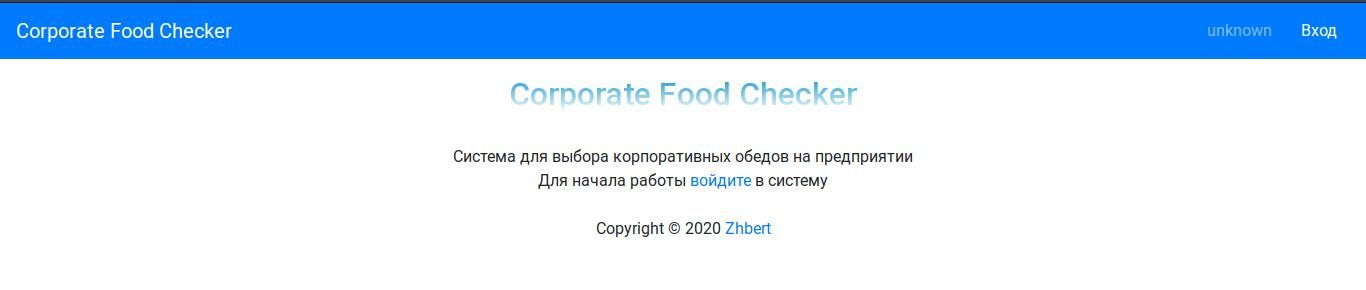
\includegraphics[width=1\linewidth]{001}}
\caption{Главная страница приложения}
\label{fig:image1}
\end{figure}

\begin{figure}[h]
\center{
\includegraphics[scale=0.23]{002}}
\caption{Главная страница приложения на мобильном устройстве}
\label{fig:image2}
\end{figure}

\end{document}  % КОНЕЦ ДОКУМЕНТА !